\textbf{EC} $\leg{a}{p}=a^{(p-1)/2}$ \\
\textbf{GL} $\leg{a}{p}=(-1)^{\abs{aP\cap N}}$

\thm (Quadratic Reciprocity) \\
For $p$, $q$ distinct odd primes
\[ \leg{q}{p} = \leg{p}{q} \text{ unless } p=q=3\bmod4 \]
in which case $\leg{q}{p} \neq \leg{p}{q}$.

\textbf{Equivalently,}
\[ \leg{q}{p} \leg{p}{q} = (-1)^{(p-1)(q-1)/4} \]
\pf $P$, $N$ \quad $Q$, $M$ \\
$\leg{q}{p}=(-1)^{\abs{qP\cap N}}$ \\
$\abs{qP\cap N}={}$\# of $x$ in $P$ such that $qx\in N$ as elements in $U_p$ \\
$qx-py\in N$ for some $y\in\Z$
\begin{align*}
qx - py &\iff py - qx \in P \\
&\iff 1 \leq py - qx \leq \frac{p-1}{2} \\
&\iff 0 < py - qx < \frac{p}{2} \\
&\iff qx < py < qx + \frac{p}{2} \\
&\iff \frac{q}{p}x < y < \frac{q}{p}x + \frac12
\end{align*}
\[ 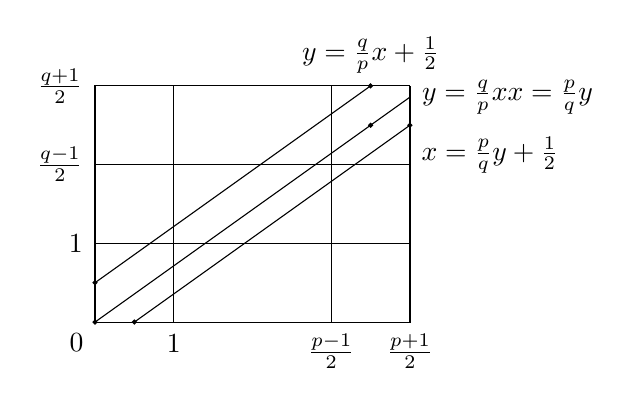
\begin{tikzpicture}
\draw(0,0)to(4,0)to(4,3);
\draw(0,0)to(0,3)to(4,3);
%\draw(0,0)to(7/2,5/2);
\draw(0,0)to(4,4*5/7);
\draw(1,0)to(1,3);
\draw(3,0)to(3,3);
\draw(0,1)to(4,1);
\draw(0,2)to(4,2);
\draw(0,1/2)to(7/2,3);
\draw(1/2,0)to(4,5/2);
\node[circle,draw,fill,color=black,inner sep=0.5pt,label=below left:$0$]at(0,0){};
\node[circle,inner sep=0.5pt,label=below:$1$]at(1,0){};
\node[circle,inner sep=0.5pt,label=left:$1$]at(0,1){};
\node[circle,inner sep=0.5pt,label=below:$\frac{p-1}{2}$]at(3,0){};
\node[circle,inner sep=0.5pt,label=below:$\frac{p+1}{2}$]at(4,0){};
\node[circle,inner sep=0.5pt,label=left:$\frac{q-1}{2}$]at(0,2){};
\node[circle,inner sep=0.5pt,label=left:$\frac{q+1}{2}$]at(0,3){};
\node[circle,inner sep=0.5pt,label=right:{$y=\frac{q}{p}x\co x=\frac{p}{q}y$}]at(4,4*5/7){};
\node[circle,draw,fill,color=black,inner sep=0.5pt]at(0,1/2){};
\node[circle,draw,fill,color=black,inner sep=0.5pt]at(1/2,0){};
\node[circle,draw,fill,color=black,inner sep=0.5pt]at(7/2,5/2){};
\node[circle,draw,fill,inner sep=0.5pt,label=above:{$y=\frac{q}{p}x+\frac{1}{2}$}]at(7/2,3){};
\node[circle,draw,fill,inner sep=0.5pt,label=below right:{$x=\frac{p}{q}y+\frac{1}{2}$}]at(4,5/2){};
\end{tikzpicture} \]
\[ \therefore\abs{qP\cap N} = \text{\# of $(x,y)\in R$} = \brack[\Big]{1,\frac{p-1}{2}}\times\brack[\Big]{1,\frac{q-1}{2}} \subseteq \Z^2 \]
strictly between $y=\frac{q}{p}x$ and $y=\frac{q}{p}x+\frac12$.

Similarly $\abs{pQ\cap M}=\text{\# of $(x,y)\in R$}$ strictly between
\[ x = \frac{p}{q} y \text{ and } x = \frac{p}{q} y + \frac12 . \]
Note that since $\gcd(p,q)=1$, there are no points in $R$ on the line $y=\frac pqx$. \\
We have
\[ \leg{q}{p} \leg{p}{q} = (-1)^{\abs{qP\cap N}+\abs{pQ\cap M}} \]
$\abs{qP\cap N}+\abs{pQ\cap M}=\text{\# of $(x,y)\in R$}$ between $y=\frac{q}{p}x+\frac12$, $x=\frac{p}{q}y+\frac12$. \\
These lines are symmetric in $R$. \\
$\therefore\abs{qP\cap N}+\abs{pQ\cap M}=\text{\# of $(x,y)$ in $R$}-2(\text{\# of $(x,y)$ in $R$ with $y\geq\frac{q}{p}+\frac12$})$
\begin{align*}
\therefore(-1)^{\abs{qP\cap N}+\abs{pQ\cap M}}&=(-1)^{\text{\# of $(x,y)$ in $R$}} \\
&= (-1)^{(\frac{p-1}{2})(\frac{q-1}{2})} \\
&= (-1)^{(p-1)(q-1)/4}
\end{align*}
\eg Show that for an odd prime $p$,
\begin{align*}
-1 \in Q_p &\iff p = 1 \bmod 4 \\
2 \in Q_p &\iff p = \pm 1 \bmod 8 \\
-2 \in Q_p &\iff p = 1, 3 \bmod 8 \\
3 \in Q_p &\iff p = \pm 1 \bmod 12 \\
&\eqvdots
\end{align*}
\soln By Euler's criterion,
\[ \leg{-1}{p} = (-1)^{(p-1)/2} = \begin{cases}
1 & \text{if $\frac{p-1}{2}$ is even} \\
-1 & \text{if $\frac{p-1}{2}$ is odd}
\end{cases} = \begin{cases}
1 & \text{if $p=1\bmod4$} \\
-1 & \text{if $p=3\bmod4$}
\end{cases} \]
By Gauss' Lemma
\[ \leg{2}{p} = (-1)^{\abs{2P\cap N}} \]
\textbf{Case 1:}
$p=1\bmod4$ (so $\frac{p-1}{2}$ is even),
\begin{align*}
P&=\brace[\Big]{1,2,\dotsc,\frac{p-1}{4},\frac{p+3}{4},\dotsc,\frac{p-1}{2}} \\
2P&=\underset{\in P}{\brace[\Big]{2,4,\dotsc,\frac{p-1}{2}}}\cup\underset{\in N}{\brace[\Big]{\frac{p+3}{2},\dotsc,p-1}} \\
\text{So } \abs{2P\cap P} &= \frac{p-1}{4} \\
\abs{2P\cap N} &= \frac{p-1}{2}-\frac{p-1}{4} = \frac{p-1}{4} \\
\therefore \leg{2}{p} &= (-1)^{(p-1)/4} \\
&= \begin{cases}
1 & \text{if $\frac{p-1}{2}$ is even} \\
-1 & \text{if $\frac{p-1}{4}$ is odd}
\end{cases} \\
&= \begin{cases}
1 & \text{if $p=1\bmod8$} \\
-1 & \text{if $p=5\bmod8$}
\end{cases}
\end{align*}
\textbf{Case 2:}
$p=3\bmod4=3,7\bmod8$ (so $\frac{p-1}{2}$ is odd)
\begin{align*}
P &= \brace[\Big]{1,2,\dotsc,\frac{p-3}{4},\frac{p+1}{4},\dotsc,\frac{p-1}{2}} \\
2P &= \underset{\in P}{\brace[\Big]{2,4,\dotsc,\frac{p-3}{2}}}\cup\underset{\in N}{\brace[\Big]{\frac{p+1}{2},\dotsc,p-1}}
\end{align*}
So $\abs{2P\cap P}=\frac{p-3}{4}$, $\cap{2P\cap N}=\frac{p-1}{2}-\frac{p-3}{4}=\frac{p+1}{4}$
\begin{gather*}
\therefore \leg{2}{p} = (-1)^{\abs{2P\cap N}} = (-1)^{(p+1)/4} = \begin{cases}
1 & \text{if $\frac{p+1}{4}$ is even} \\
-1 & \text{if $\frac{p+1}{4}$ is odd}
\end{cases} = \begin{cases}
1 & \text{if $p=7\bmod8$} \\
-1 & \text{if $p=3\bmod8$}
\end{cases} \\
\therefore \leg{2}{p} = \begin{cases}
1 & \text{if $p=1,7\bmod8$} \\
-1 & \text{if $p=3,5\bmod8$}
\end{cases}
\end{gather*}
Is $-2\in Q_p$?
\begin{gather*}
\leg{-2}{p} = \leg{-1}{p}\leg{2}{p} \\
\leg{-1}{p} = \begin{cases}
1 & p=1\bmod4\text{, i.e., }p=1,5\bmod8 \\
-1 & p=3\bmod4\text{, i.e., }p=3,7\bmod8
\end{cases} \\
\leg{2}{p} = \begin{cases}
1 & p=1,7\bmod8 \\
-1 & p=3,5\bmod8
\end{cases} \\
\therefore \begin{array}{c|cccc}
p & 1 & 3 & 5 & 7 \\ \hline
\leg{-2}{p} & 1 & 1 & -1 & -1
\end{array} \\
\therefore \leg{-2}{p} = \begin{cases}
1 & p=1,3\bmod8 \\
-1 & p=5,7\bmod8
\end{cases}
\end{gather*}
Is $3\in Q_p$? $3\notin Q_3$, so let $p>3$.
\begin{align*}
\leg{3}{p} &= \begin{cases}
\leg{p}{3} & p=1\bmod4 \\
-\leg{p}{3} & p=3\bmod4
\end{cases} \\
&= \begin{cases}
\begin{cases}
1 & p=1\bmod4,p=1\bmod3\text{, i.e., }p=1\bmod12 \\
-1 & p=1\bmod4,p=2\bmod3\text{, i.e., }p=5\bmod12
\end{cases} \\
\begin{cases}
1 & p=3\bmod4,p=2\bmod3\text{, i.e., }p=11\bmod12 \\
-1 & p=3\bmod4,p=1\bmod3\text{, i.e., }p=7\bmod12
\end{cases}
\end{cases} \\
\therefore \leg{3}{p} &= \begin{cases}
1 & \text{if $p=1,11\bmod12$} \\
-1 & \text{if $p=5,7\bmod12$}
\end{cases}
\end{align*}
\eg\begin{enumerate}
\item Is $7\in Q_{43}$?
\item Is $136\in Q_{421}$?
\item Is $468\in Q_{697}$?
\end{enumerate}
For (1), we give 4 solutions: \\
In $U_{43}$,
\[ \scriptsize\begin{array}{c|cccccccccccccccccccccc}
x & 1 & 2 & 3 & 4 & 5 & 6 & 7 & 8 & 9 & 10 & 11 & 12 & 13 & 14 & 15 & 16 & 17 & 18 & 19 & 20 & 21 & 22 \\ \hline
x^2 & 1 & 4 & 9 & 16 & 25 & 36 & 6 & 21 & 38 & 14 & 35 & 15 & 40 & 24 & 10 & 41 & 31 & 23 & 17 & 13 & 11 & 11 \\
7^x & 7 & 6 & -1 & -7 & -6 & -1 & & & -1 & & & 1 & & & -1 & & & 1 & & & -1 & \\
7x & 7 & 14 & 21 & -15 & -8 & -1 & 6 & 13 & 20 & -16 & -9 & -2 & 5 & 12 & 19 & -17 & -10 & -3 & 4 & 11 & 18 & 
\end{array} \]
squares $\implies7\notin Q_{43}$ \\
E.C.: $\leg{7}{43}=7^{21}=-1$ \\
G.L.: $(-1)^{\abs{7P\cap Q}}=(-1)^9=-1$ \\
Q.R.: $\leg{7}{43}=-\leg{43}{7}=-\leg{1}{7}=-1$
